\chapter{Activity Flow glyphs}
\label{chp:af:glyphs}

\section{Overview}

To set the stage for what follows in this chapter, we first give a brief overview of some of the concepts in the \AF notation with the help of an example shown in \fig{eg1}.

\begin{figure}[H]
  \centering
  \vspace*{-0.75em}
%  \includegraphics[scale=0.8]{examples/MAPK-only}
  \caption{}
  \label{fig:eg1}
\end{figure}



\section{Controlled vocabularies used in \SBGNAFLone}\label{af:sec:CVs}

%%%%%%%%%%%%%%%%%%%%%%%%%%%%%%%%%%%%%%%%%%%%%%%%%%%%%%%%%%%%%%%%%%%%%%
%%%%                   Controlled vocabularies
%%%%%%%%%%%%%%%%%%%%%%%%%%%%%%%%%%%%%%%%%%%%%%%%%%%%%%%%%%%%%%%%%%%%%%

\color{red}
What controlled vocabulary should we use? SBO? GO molecular function?
\normalcolor

Some glyphs in SBGN \AF can contain particular kinds of textual annotations conveying information relevant to the purpose of the glyph.  These annotations are \glyph{units of information} (\sect{af:unitInfo}).  An example is in the case of a compartment, which can have a unit of information conveying physical characteristics of the compartment .

The text that appears as the unit of information decorating an Activity Node (AN) od Container Node (CN) must in most cases be prefixed with a controlled vocabulary term indicating the type of information being expressed. Without the use of controlled vocabulary prefixes, it would be necessary to have different glyphs to indicate different classes of information; this would lead to an explosion in the number of symbols needed. 

In the rest of this section, we describe the controlled vocabularies (CVs) used in \SBGNAFLone. Some CV terms are predefined by SBGN, but unless otherwise noted, they are not the only terms permitted. Authors may use other CV values not listed here, but in such cases, they should explain the term's meanings in a Figure legend or other text accompanying the map.

\subsection{Activity node material types}
\label{sec:af:material-types-cv}

The material type of an AFN indicates its chemical structure.  A list of common material types is shown in \tab{af:material-types-cv}, but others are possible.  The values are to be taken from the \sbo (\sbourl), specifically from the branch having identifier \sboid{SBO:0000240} ($\!$\emph{material entity} under \emph{participant}$\rightarrow$\emph{physical participant}).  The labels are defined by \SBGNAFLone.

\begin{table}[h]
  \centering
  \begin{tabular}{l>{\ttfamily}l>{\ttfamily}l}
    \toprule
    \textbf{Name}              & \textbf{\rmfamily Label} & \textbf{\rmfamily SBO term} \\
    \midrule
    Non-macromolecular ion     & mt:ion  & SBO:0000327\\
    Non-macromolecular radical & mt:rad  & SBO:0000328\\
    Ribonucleic acid           & mt:rna  & SBO:0000250\\
    Deoxribonucleic acid       & mt:dna  & SBO:0000251\\
    Protein                    & mt:prot & SBO:0000297\\
    Polysaccharide             & mt:psac & SBO:0000249\\
    \bottomrule
  \end{tabular}
  \caption{A sample of values from the \emph{material types} controlled
    vocabulary (\sect{af:material-types-cv}).}
  \label{tab:af:material-types-cv}
\end{table}

The material types are in contrast to the \emph{conceptual types} (see below).  The distinction is that material types are about physical composition, while conceptual types are about roles.  For example, a strand of RNA is a physical artifact, but its use as messenger RNA is a role.

\subsection{Activity node conceptual types}
\label{sec:af:conceptual-types-cv}

An AFN's \emph{conceptual type} indicates its function within the context of a given \AF.  A list of common conceptual types is shown in \tab{af:conceptual-types-cv}, but others are possible.  The values are to be taken from the \sbo (\sbourl), specifically from the branch having identifier \sboid{SBO:0000241} ($\!$\emph{conceptual entity} under \emph{participant}$\rightarrow$\emph{physical participant}).  The labels are defined by \SBGNAFLone.

\begin{table}[h]
  \centering
  \begin{tabular}{l>{\ttfamily}l>{\ttfamily}l}
    \toprule
    \textbf{Name}              & \textbf{\rmfamily Label} & \textbf{\rmfamily SBO term} \\
    \midrule
    Gene                      & ct:gene   & SBO:0000243\\
    Transcription start site  & ct:tss    & SBO:0000329\\
    Gene coding region        & ct:coding & SBO:0000335\\
    Gene regulatory region    & ct:grr    & SBO:0000369\\
    Messenger RNA             & ct:mRNA   & SBO:0000278\\
    \bottomrule
  \end{tabular}
  \caption{A sample of values from the \emph{conceptual types} vocabulary
    (\sect{af:conceptual-types-cv}).}
  \label{tab:af:conceptual-types-cv}
\end{table}

\subsection{Physical characteristics of compartments}
\label{sec:af:physical-characteristics-cv}

\SBGNAFLone defines a special unit of information for describing certain common physical characteristics of compartments.  \tab{af:physical-characteristics-cv} lists the particular values defined by \SBGNAFLone.  The values correspond to the \sbo branch with identifier \sboid{SBO:0000255} (\emph{physical characteristic} under \emph{quantitative parameter}).

\begin{table}[h]
  \centering
  \begin{tabular}{l>{\ttfamily}l>{\ttfamily}l}
    \toprule
    \textbf{Name}   & \textbf{\rmfamily Label} & \textbf{\rmfamily SBO term} \\
    \midrule
    Temperature   & pc:T  & SBO:0000147\\
    Voltage       & pc:V  & SBO:0000259\\
    pH            & pc:pH & SBO:0000304\\
    \bottomrule
  \end{tabular}
  \caption{A sample of values from the \emph{physical
      characteristics} vocabulary (\sect{af:physical-characteristics-cv}).}
  \label{tab:af:physical-characteristics-cv}
\end{table}

%\subsection{Cardinality}
%\label{sec:af:cardinality-cv}
%
%\SBGNAFLone defines a special unit of information usable on multimers for describing the number of monomers composing the multimer.  \tab{af:cardinality-cv} shows the way in which the values must be written.  Note that the value is a unitary number, and not (for example) a range.  There is no provision in \SBGNAFLone for specifying a range in this context because it leads to problems of entity identifiability.
%
%\begin{table}[h]
%  \centering
%  \begin{tabular}{l>{\ttfamily}l>{\ttfamily}l}
%    \toprule
%    \textbf{Name}   & \textbf{\rmfamily Label} & \textbf{\rmfamily SBO term} \\
%    \midrule
%    cardinality    & N:\#  & SBO:0000364\\
%    \bottomrule
%  \end{tabular}
%  \caption{The format of the possible values for the
%    \emph{cardinality} unit of information
%    (\sect{af:cardinality-cv}).  Here, \texttt{\#} stands for the
%    number; for example, ``\texttt{N:5}''.}
%  \label{tab:af:cardinality-cv}
%\end{table}


%%%%%%%%%%%%%%%%%%%%%%%%%%%%%%%%%%%%%%%%%%%%%%%%%%%%%%%%%%%%%%%%%%%%%%
%%%%                   Activity nodes
%%%%%%%%%%%%%%%%%%%%%%%%%%%%%%%%%%%%%%%%%%%%%%%%%%%%%%%%%%%%%%%%%%%%%%

\section{Activity nodes}\label{sec:af:ANs}

An \emph{Activity node} (AN) represents the activity of an entity or an entity pool, but not the entities themselves. For instance, multiple activity nodes can be used to represent different activities of a particular entity, while one activity node can be used to represent the activity of a complex multimer. In addition to activities of material entities, \SBGNAFLone represents activity from a conceptual entity: \emph{phenotype}.  Auxiliary units, such as \emph{units of information}, can be used to indicate the material property of the activity source.  Each activity is displayed only once in a particular compartment.


\subsection{Glyph: \glyph{Biological activity}}
\label{sec:af:biologicalActivity}


\SBGNAFLone uses one glyph to represent activities from all biological entities, collectively they are called \emph{biological activity}. The nature of the molecule that the activity comes from, eg., simple chemical or macromolecule, can be encoded in the \emph{units of information} (\sect{af:unitInfo}). 

It should be noted that the \emph{biological activity} is not equivalent to a biological entity per se.  A biological activity can come from one biological entity, a part of an entity, or a combination of  them.  It is up to the users how to represent it in their diagram.  For example, a protein kinase receptor such as an EGF receptor, has two activities, the binding activity that allows the extracellular part of the receptor to bind to the ligand, and the kinase activity that is capable of phosphorylating the downstream protein and initiating the intracellular signaling.  The user can choose to use two nodes to represent each activity, or to use one node to represent the overall "EGF receptor activity".

\begin{glyphDescription}

\glyphSboTerm SBO:

\glyphContainer An \glyph{biological activity} is represented by a rectangle, as shown in \fig{af:biologicalActivity}.

\glyphLabel An \glyph{biological activity} is identified by a label placed in an unbordered box containing a string of characters.  The characters can be distributed on several lines to improve readability, although this is not mandatory.  The label box must be attached to the center of the container.  The label may spill outside of the container.

\glyphAux A \glyph{biological activity} can carry a \glyph{unit of information} (\sect{af:unitInfo}), which can provide information such as the nature of the entity from which the activity originated.  Specific glyphs are used to represent different types of entities (\sect{af:unitInfo}).  The center of the bounding box of a \glyph{unit of information} is located on the mid-line of the border of the macromolecule.

\end{glyphDescription}

\begin{figure}[H]
  \centering
  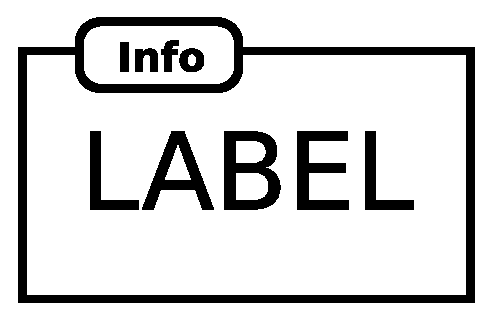
\includegraphics[scale = 0.5]{images/biologicalActivity}
  \caption{The \AF glyph for \glyph{biological activity}.}
  \label{fig:af:biologicalActivity}
\end{figure}

%%%    Process

\subsection{Glyph: \glyph{Process}}
\label{sec:af:process}

In \SBGNAFLone, a \emph{process} is used to represent a conceptual outcome of a sequential series of actions, motions, or occurrences, such as chemical reactions, that usually involve multiple biological activities from multiple entities.

Although a \emph{process} may also have implications of biological activities, it is different from the glyph \emph{biological activity} in that the latter is the activity from a defined EPN.



\begin{glyphDescription}

\glyphSboTerm SBO:0000375 ! process

\glyphContainer A \glyph{process} is represented by a double-lined rectangle, as shown in \fig{af:process}. 

\glyphLabel A \glyph{process} is identified by a label placed in an unbordered box containing a string of characters.  The characters can be distributed on several lines to improve readability, although this is not mandatory.  The label box must be attached to the center of the container.  The label may spill outside of the container.

\glyphAux None.

\end{glyphDescription}

\begin{figure}[H]
  \centering
  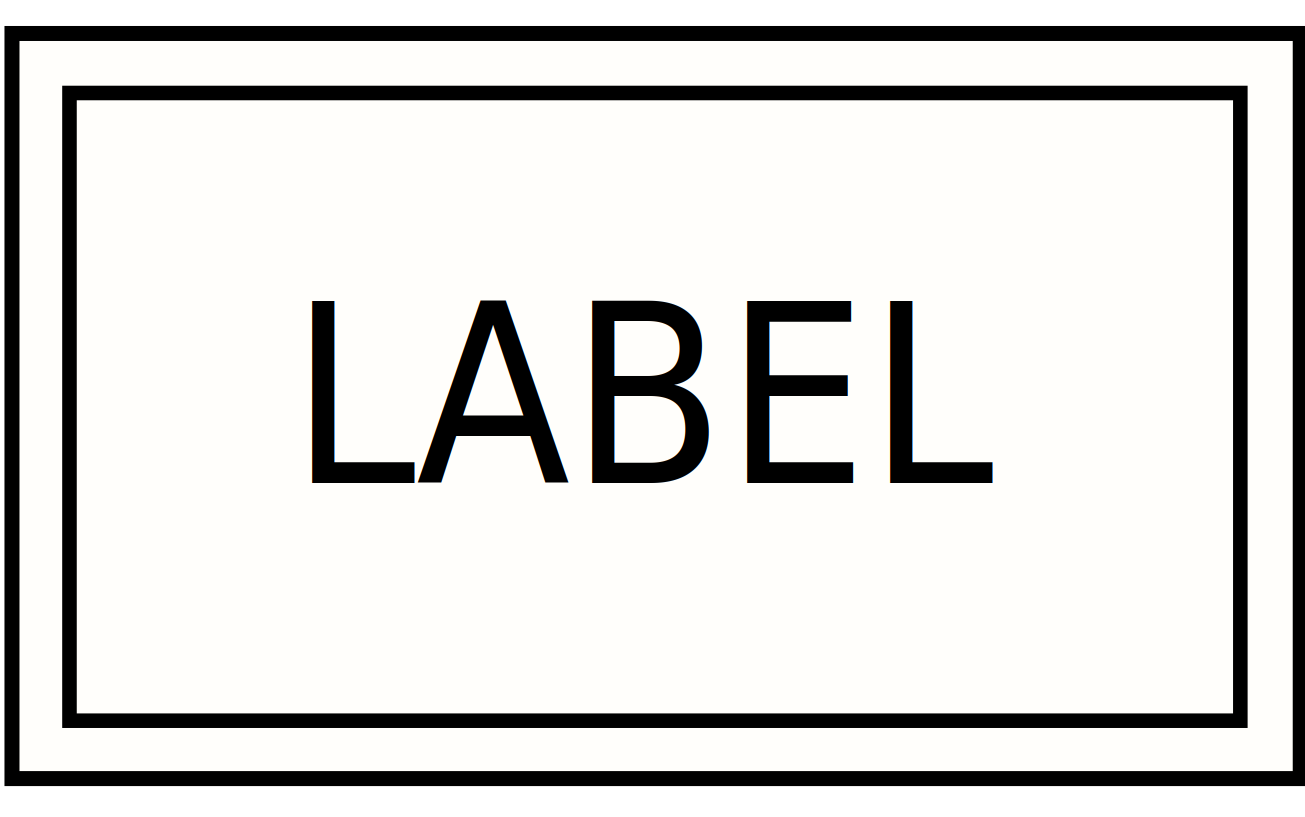
\includegraphics[scale=0.1]{images/process}
  \caption{The \AF glyph for \glyph{process}.}
  \label{fig:af:process}
\end{figure}

\subsection{Glyph: \glyph{Phenotype}}
\label{sec:af:phenotype}

A phenotype is a type of biological process.  In SBGN, \emph{phenotype} is used to show the observable or measurable outcome of the network.  It is usually the end-point(s) of the network, i.e., it cannot be used as the start of an arc.

\begin{glyphDescription}

\glyphSboTerm
SBO:0000358 ! phenotype

\glyphIncoming Zero or more \glyph{influence} arcs (\sect{af:arcs}).

\glyphOutgoing None.

\glyphContainer A \glyph{phenotype} is represented by an elongated hexagon, as illustrated in \fig{af:phenotype}.

\glyphLabel A \glyph{phenotype} is identified by a label placed in an unbordered box containing a string of characters.  The characters can be distributed on several lines to improve readability, although this is not mandatory.  The label box must be attached to the centre of the \glyph{phenotype} container.  The label may spill outside of the container.

\glyphAux None.

\end{glyphDescription}

\begin{figure}[H]
  \centering
  \includegraphics[scale = 1]{images/build/phenotype.pdf}
  \caption{The \AF glyph for \glyph{phenotype}.}
  \label{fig:af:phenotype}
\end{figure}


%%%%%%%%%%%%%%%%%%%%%%%%%%%%%%%%%%%%%%%%%%%%%%%%%%%%%%%%%%%%%%%%%%%%%%
%%%%                   Auxiliary units
%%%%%%%%%%%%%%%%%%%%%%%%%%%%%%%%%%%%%%%%%%%%%%%%%%%%%%%%%%%%%%%%%%%%%%

\section{Auxiliary units}\label{sec:af:AUs}

\subsection{Glyph: \glyph{Unit of information for Biological activity}}
\label{sec:af:unitInfo}

When representing biological activities, it is often useful to illustrate the nature of the entity where the activity is originated, e.g., whether the activity is from a macromolecule (protein or nucleic acid), or from a chemical compound.  The \SBGNAFLone \glyph{unit of information} is used to add such information to a glyph.  It represents the information in two ways.  First, different symbols are used to represent the nature of the entity where the activity is from, e.g., macromolecule, nucleic acid feature, or complex.  These symbols are identical to the \glyph{entity pool node} symbols in SBGN \PDl.  Second, names of the entity (gene names, protein names) are usually provided as labels in the \glyph{unit of information} container.

\begin{glyphDescription}

\glyphSboTerm Not applicable.

\glyphContainer A unit of information is represented by containers of different shapes, depending on the nature of the entity where the biological activity is from. There are a total of six types of unit of information, as shown in \fig{af:unitInfo}.   Below is a summary of the six glyphs.

\begin{description}
\item[A.] Macromolecule -- Macromolecules are biochemical substances that are built up from the covalent linking of pseudo-identical units. Examples of macromolecules include proteins, nucleic acids (RNA, DNA), and polysaccharides (glycogen, cellulose, starch, etc.).  
A unit of information of a macromolecule is represented by a rectangle with rounded corners, as illustrated in (A) of \fig{af:unitInfo}.  This container is used to decorate a biological activity that is originated from a macromolecule, such as a protein, a nucleic acid, or a complex sugar.

\item[B.] Nucleic acid feature -- The nucleic acid feature construct in SBGN is meant to represent a fragment of a macromolecule carrying genetic information. A unit of information of a nucleic acid feature is represented by a rectangle whose bottom half has rounded corners, as shown in (B) of \fig{af:unitInfo}.

\item[C.] Simple chemical -- A simple chemical is a chemical compound that is not formed by the covalent linking of pseudo-identical residues. Examples of simple chemicals are an atom, a monoatomic ion, a salt, a radical, a solid metal, a crystal, etc. 
A unit of information of a simple chemical is represented by a “stadium” shape, that is two semicircles of the same
radius joined by parallel line segments, as shown in (C) of \fig{af:unitInfo}. If desired the parallel line segments can have zero length, and the shape is then identical to a circle. To avoid confusion with the unspecified entity (shown in D of (\fig{af:unitInfo}), this form of the glyph must remain a circle and cannot be deformed into an ellipse.

\item[D.] Unspecified entity -- An unspecified entity is used to represent the entity type that is unknown or simply not relevant to the purposes of the map. This arises, for example, when the existence of the entity has been inferred indirectly, or when the entity is merely a construct introduced for the needs of a map, without direct biological relevance. A unit of information of an unspecified entity is represented by an elliptic container, as shown in (D) of \fig{af:unitInfo}.  It is used to decorate a biological activity that is originated from an unspecified entity.

\item[E.] Complex -- A complex represents a biochemical entity composed of other biochemical entities, whether macromolecules, simple chemicals, or other complexes. The resulting entity may 
have its own identity, properties and function in an SBGN map. A unit of information of a complex is represented by an octagon as shown in (E) of \fig{af:unitInfo}.  It is used to decorate a biological activity that is originated from a complex.

\item[F.] Perturbation -- Biochemical networks can be affected by external influences. Those influences can be well-defined physical perturbations, such as a light pulse or a change in temperature; they can also be more complex and not well-defined phenomena, for instance, glucose deprivation, stress.  A unit of information of a perturbation is represented by a modified hexagon
having two opposite concave faces, as illustrated in F of  \fig{af:unitInfo}.  It is used to decorate a biological activity when it is originated from a perturbation.
\end{description}

\begin{figure}[H]
  \centering
  \includegraphics[scale = 0.7]{src/images/build/unit_info_ba.pdf}
  \caption{The \AF glyph for \glyph{unit of information}.}
  \label{fig:af:unitInfo}
\end{figure}

\begin{figure}[H]
  \centering
  \includegraphics[scale = 1]{images/build/unit_info_sample.pdf}
  \caption{Examples of \glyph{unit of information} used on \glyph{biological activity node} to indicate that the \emph{Twist-1 activity} is from a \emph{nucleic acid feature} or a \emph{macromolecule}, or a \emph{transcription factor activity} from an \emph{unspecified} entity.}
  \label{fig:af:unitofinfo}
\end{figure}

\fig{af:unitofinfo} shows examples taken from \fig{af:1}, where \emph{units of information} is used on Activity Nodes to illustrate the properties of the entities from which the activities originate.

The long side of the glyphs above (except for simple chemical) should be oriented parallel to the border of the \glyph{AN} being annotated by the \glyph{unit of information}. The centre of the bounding box of a \glyph{state of information} should be located on the mid-line of the border of the \glyph{AN}.

\glyphLabel A \glyph{unit of information} is not required to carry any label.   If a label is desired, it should be placed in an unbordered box containing a string of characters. The characters can be distributed on several lines to improve readability, although this is not mandatory.  The label box must be attached to the centre of the container. The label may spill outside of the container.  The label defines the information carried by the \glyph{unit of information}.

\glyphAux A \glyph{unit of information} does not carry any auxiliary items.

\end{glyphDescription}

\subsection{Glyph: \glyph{Unit of information for Compartment}}
\label{sec:af:unitInfoComp}

A \emph{unit of information} can be used to decorate a compartment to convey information about physical characteristics of the compartments (\sect{af:physical-characteristics-cv}). 

\begin{glyphDescription}

\glyphSboTerm Not applicable.

\glyphContainer A \emph{unit of information} for compartment is represented by a rectangle as shown in \fig{compunitInfo}.  The long side of the rectangle should be oriented parallel to the border of the \glyph{compartment} being annotated by the \glyph{unit of information}. The centre of the bounding box of a \glyph{unit of information} should be located on the mid-line of the border of the \glyph{compartment}.

\begin{figure}[H]
  \centering
  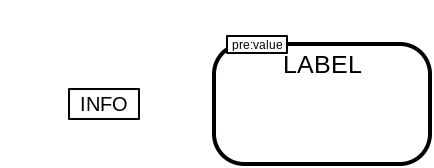
\includegraphics[scale = 0.7]{images/build/unit_info_comp.pdf}
  \caption{The \AF glyph for \glyph{unit of information}.}
  \label{fig:compunitInfo}
\end{figure}

\glyphLabel A \glyph{unit of information} is identified by a label placed in an unbordered box containing a string of characters.  The characters can be distributed on several lines to improve readability, although this is not mandatory.  The label box must be attached to the centre of the container.  The label may spill outside of the container.

The label defines the information carried by the \glyph{unit of information}.  For certain predefined types of information for the compartment, such as physical characteristics, SBGN defines specific prefixes that must be included in the label to indicate the type of information in question.  The controlled vocabularies predefined in \SBGNAFLone are described in \sect{af:physical-characteristics-cv} and summarized in the following list:

\begin{center}
  \begin{itemize}\setlength{\parskip}{0ex}
  \item{pc:T} Temperature (SBO:0000147)
  \item{pc:V} Voltage (SBO:0000259)
  \item{pc:pH} pH (SBO:0000304)
  \end{itemize}
\end{center}

    
\glyphAux A \glyph{unit of information} does not carry any auxiliary items.  

\end{glyphDescription}



\input{src/submap_terminal.tex}

%%%%%%%%%%%%%%%%%%%%%%%%%%%%%%%%%%%%%%%%%%%%%%%%%%%%%%%%%%%%%%%%%%%%%%
%%%%                   Container nodes
%%%%%%%%%%%%%%%%%%%%%%%%%%%%%%%%%%%%%%%%%%%%%%%%%%%%%%%%%%%%%%%%%%%%%%

\section{Container nodes}
\label{sec:af:CNs}

\glyph{Containers} are SBGN constructions that contain one or several other SBGN constructs.  In \SBGNAFLone \glyph{compartment} is the only container node.

A compartment is a logical or physical structure where the function or activity is located.  At the moment, an activity can only belong to one compartment. Therefore, the ``same'' biochemical activities located in two different compartments are in fact, two different activities, and should be represented separately.

\begin{glyphDescription}

\glyphSboTerm  SBO:0000289 ! functional compartment

\glyphIncoming None.

\glyphOutgoing Zero or more \glyph{equivalence arcs} (\sect{equivalenceArc}).

\glyphContainer A compartment is represented by a surface enclosed in a continuous border or located between continuous borders. These borders should be noticeably thicker than the borders of the ANs. A compartment can take \textbf{any} geometry. A compartment must always be entirely enclosed.

\glyphLabel The identification of the compartment is carried by an unbordered box containing a string of characters. The characters can be distributed on several lines to improve readability, although this is not mandatory. The label box can be attached anywhere in the container box. Note that the label can spill over from the container box.

\glyphAux A \glyph{compartment} can carry a certain number of \glyph{units of information}, that will add information, for instance, about the physical environment, such as pH, temperature or voltage, see \sect{af:unitInfoComp}.  The centre of the bounding box of a \glyph{unit of information} must lie on the border of the compartment.

\end{glyphDescription}

\begin{figure}[H]
  \centering
  \includegraphics[scale = 1]{images/build/compartment.pdf}
  \caption{The \AF glyph for \glyph{compartment}.}
  \label{fig:af:compartment}
\end{figure}

It is important to note that a compartment never contains another compartment. To allow more aesthetically pleasing and understandable diagrams, compartments are allowed to overlap each other visually, but it must be kept in mind that this does not mean one compartment contains part or entire of the other compartment.  \fig{overlap} shows three semantically equivalent placements of compartments:

\begin{figure}[H]
  \centering
  \includegraphics[scale = 0.4]{images/build/compartment_overlapping_example.pdf}
  \caption{Overlapped compartments are permitted, but the overlap does not imply containment.}
  \label{fig:overlap}
\end{figure}



%%%%%%%%%%%%%%%%%%%%%%%%%%%%%%%%%%%%%%%%%%%%%%%%%%%%%%%%%%%%%%%%%%%%%%
%%%%                  Arcs
%%%%%%%%%%%%%%%%%%%%%%%%%%%%%%%%%%%%%%%%%%%%%%%%%%%%%%%%%%%%%%%%%%%%%%

\section{Modulation arcs}\label{sec:af:arcs}

Modulation arcs are lines that link ANs together.  The symbols attached to their end extremities indicate their semantics.  The modulation arcs can be used to represent direct influence from one activity to another, such as nicotine to nicotinic acetylecholine receptor activity, or indirect influence.

\subsection{Glyph: \glyph{Positive influence}}
\label{sec:af:positive_infl}

A \emph{positive influence} represents that an activity exerts a \textbf{positive} or \textbf{stimulating} effect on another activity.

\begin{glyphDescription}

\glyphSboTerm SBO:0000170 ! stimulation

 \glyphOrigin One \glyph{biological activity} (\sect{af:biologicalActivity}) or \glyph{logical operator} (\sect{af:logic}).
 \glyphTarget One \glyph{biological activity} (\sect{af:biologicalActivity}) or \glyph{phenotype} (\sect{af:phenotype}).
 \glyphEndPoint The target extremity of a \glyph{positive influence} carries an open arrow pointing to the target activity node (\fig{af:positiveInfl}).

\end{glyphDescription}

\begin{figure}[H]
  \centering
  \includegraphics[width = 2in]{images/build/positive_influence.pdf}
  \caption{The \AF glyph for \glyph{positive influence}.}
  \label{fig:af:positiveInfl}
\end{figure}

\begin{figure}[H]
  \centering
  \includegraphics[scale = 1]{images/build/positive_influence_example.pdf}
  \caption{An example, taken from \fig{af:1}, of \glyph{positive influence} from a \glyph{perturbation} to the nuclear hormone receptor \glyph{PPAR$\delta$.}}
  \label{fig:af:exPI}
\end{figure} 
\subsection{Glyph: \glyph{Negative influence}}
\label{sec:af:negative_infl}

A \emph{negative influence} represents that an activity exerts a \textbf{negative} or \textbf{inhibiting} effect on another activity.

\begin{glyphDescription}

\glyphSboTerm SBO:0000169 ! inhibition

 \glyphOrigin One \glyph{biological activity} (\sect{af:biologicalActivity}) or \glyph{logical operator} (\sect{af:logic}).
 \glyphTarget One \glyph{biological activity} (\sect{af:biologicalActivity}) or \glyph{phenotype} (\sect{af:phenotype}).
 \glyphEndPoint The target extremity of a \glyph{negative influence} carries a bar perpendicular to the arc (\fig{af:negativeInfl}).

\end{glyphDescription}

\begin{figure}[H]
  \centering
  \includegraphics[width = 2in]{images/build/negative_influence.pdf}
  \caption{The \AF glyph for \glyph{negative influence}.}
  \label{fig:af:negativeInfl}
\end{figure}

\begin{figure}[H]
  \centering
  \includegraphics[scale=1]{images/build/negative_influence_example.pdf}
  \caption{An example, taken from \fig{af:1}, of \glyph{negative influence} from \glyph{Twist-1} protein activity to \glyph{PGC-1$\alpha$} activity.}
  \label{fig:af:ex-NI}
\end{figure} 
\subsection{Glyph: \glyph{Unknown influence}}
\label{sec:af:unknown_infl}

An \emph{unknown influence} represents that an activity affects another activity, but the exact nature of this effect is not specified or not known.

\begin{glyphDescription}

\glyphSboTerm SBO:0000168 ! control

 \glyphOrigin One \glyph{biological activity} (\sect{af:biologicalActivity}) or \glyph{logical operator} (\sect{af:logic}).
 \glyphTarget One \glyph{biological activity} (\sect{af:biologicalActivity}) or \glyph{phenotype} (\sect{af:phenotype}).
 \glyphEndPoint The target extremity of an \glyph{unknown influence} carries an open diamond (\fig{af:unknownInfl}).

\end{glyphDescription}

\begin{figure}[H]
  \centering
  \includegraphics[width = 2in]{images/build/unknown_influence.pdf}
  \caption{The \AF glyph for \glyph{unknown influence}.}
  \label{fig:af:unknownInfl}
\end{figure}

\begin{figure}[H]
  \centering
  \includegraphics[scale = 1]{images/build/unknown_influence_example.pdf}
  \caption{An example, taken from \fig{EGF}, of \glyph{unknown influence} from the adaptor protein \glyph{Cbl} to the signalling enzyme \glyph{PLC gamma.}}
  \label{fig:af:exPI}
\end{figure} 


\subsection{Glyph: \glyph{Necessary stimulation}}
\label{sec:af:trigger}
A \glyph{necessary stimulation} is an influence that has to be present for the target activity to take place (to become true).  An activity modulated by a necessary stimulation can only exist when this stimulation is true, whatever are the other influences this activity is subjected to.

\begin{glyphDescription}

\glyphSboTerm SBO:0000171 ! necessary stimulation

  \glyphOrigin Any \glyph{biological activity} (\sect{af:biologicalActivity}) or any \glyph{logical operator} (\sect{af:logic}).
 \glyphTarget Any \glyph{biological activity} (\sect{af:biologicalActivity}) or \glyph{phenotype} (\sect{af:phenotype}).
 \glyphEndPoint The target extremity of a \glyph{necessary stimulation} carries a perpendicular bar followed by an open arrow pointing to the target activity node (\fig{af:trigger}).  The bar has to be at least as long as the base of the arrowhead.

\end{glyphDescription}

\begin{figure}[H]
  \centering
  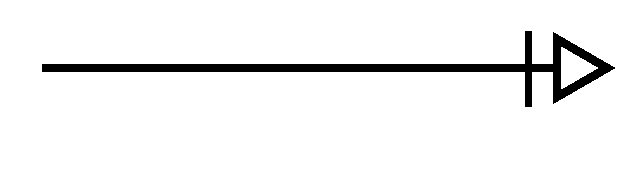
\includegraphics[width = 2in]{images/build/necessaryStimulation.pdf}
  \caption{The \AF glyph for \glyph{necessary stimulation}.}
  \label{fig:af:trigger}
\end{figure}

\begin{figure}[H]
  \centering
  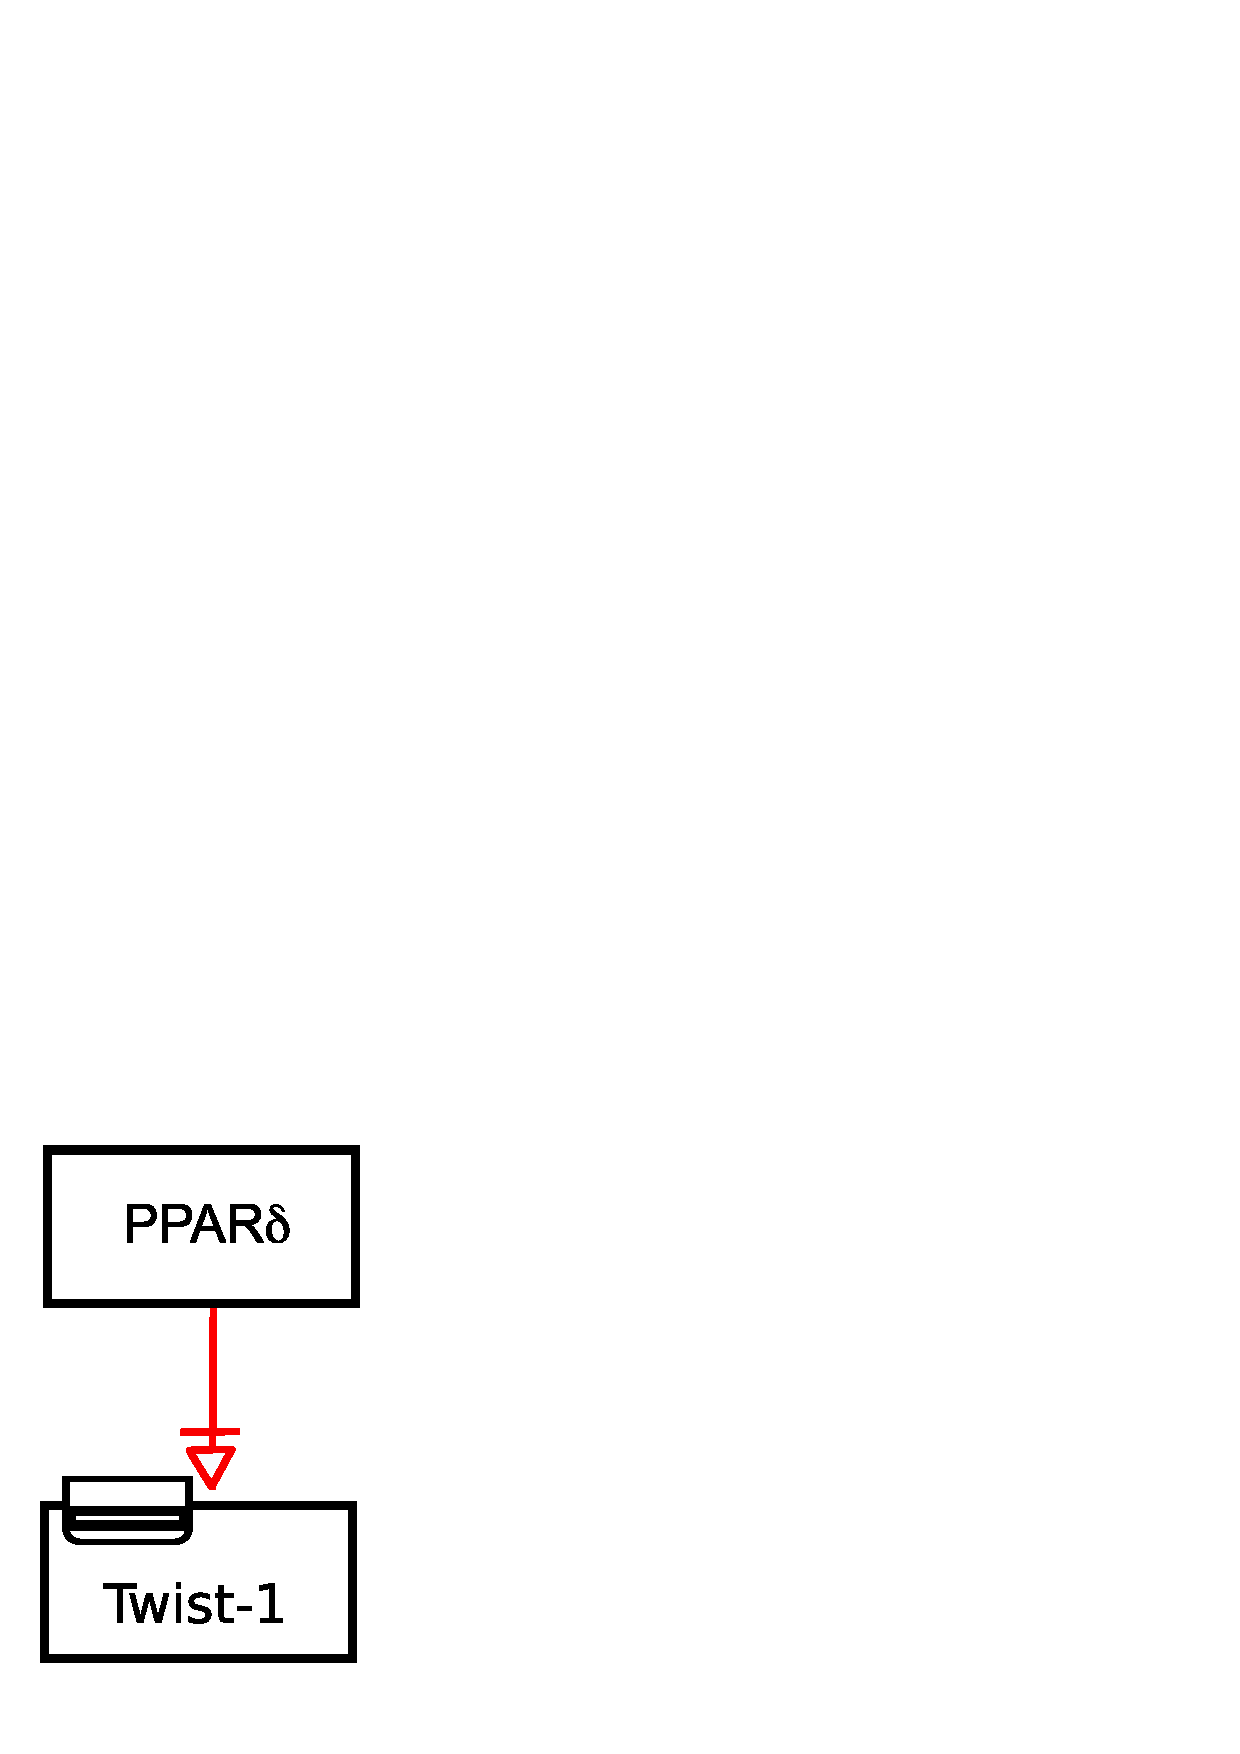
\includegraphics[width = 1.5in]{images/build/ex-necessaryStimulation.pdf}
  \caption{An example, taken from \fig{af:1}, of \glyph{necessary stimulation} where nuclear hormone receptor \glyph{PPAR $\delta$} transcription factor activity is necessary for the stimulation of the \glyph{Twist-1} gene expression. }
  \label{fig:af:ex-NS}
\end{figure}




%%%%%%%%%%%%%%%%%%%%%%%%%%%%%%%%%%%%%%%%%%%%%%%%%%%%%%%%%%%%%%%%%%%%%%
%%%%                   Logical operators
%%%%%%%%%%%%%%%%%%%%%%%%%%%%%%%%%%%%%%%%%%%%%%%%%%%%%%%%%%%%%%%%%%%%%%

\section{Logical operators}\label{sec:af:logic}

\subsection{Glyph: \glyph{And}}
\label{sec:af:and}

The glyph \glyph{and} is used to denote that all the \glyph{ANs} linked as input are necessary to influence the target activity.

\begin{glyphDescription}
 \glyphSboTerm SBO:0000173 ! and.
 \glyphIncoming One or more \glyph{logic arcs} (\sect{af:logicArc}).
 \glyphOutgoing  One \glyph{logic arc} (\sect{af:logicArc}) or one of the modulation arcs (\sect{af:arcs}).
 \glyphContainer An \glyph{and} operator is represented by a circular shape containing the word ``AND''.
The shape is linked to two ports, that are small arcs attached to the centres of opposite sides of the shape, as shown in \fig{af:and}.
The incoming \glyph{logic arcs} (\sect{af:logicArc}) are linked to the extremity of the leftmost or uppermost port, while the outgoing \glyph{logic arc} (\sect{af:logicArc}) or modulation arc (\sect{af:arcs}) is linked to the extremity of the rightmost or bottommost port.
 \glyphLabel None.
 \glyphAux None.
\end{glyphDescription}

\begin{figure}[H]
  \centering
  \includegraphics[scale = 1]{images/build/and.pdf}
  \caption{The \AF glyph for \glyph{and}. Only two inputs are represented, but more would be allowed.}
  \label{fig:af:and}
\end{figure}

\subsection{Glyph: \glyph{Or}}
\label{sec:af:or}

The output of an \glyph{or} glyph is True if at least one of its inputs is True, and False otherwise.

\begin{glyphDescription}
 \glyphSboTerm SBO:0000174 ! or.
 \glyphIncoming One or more \glyph{logic arcs} (\sect{af:logicArc}).
 \glyphOutgoing  One \glyph{logic arc} (\sect{af:logicArc}) or one of the influence arcs (\sect{af:arcs}).
 \glyphContainer An \glyph{or} operator is represented by a circular shape containing the word ``OR''.
The shape is linked to two ports, that are small arcs attached to the centres of opposite sides of the shape, as shown in \fig{af:or}.
 \glyphLabel None.
 \glyphAux None.
 \end{glyphDescription}

\begin{figure}[H]
  \centering
  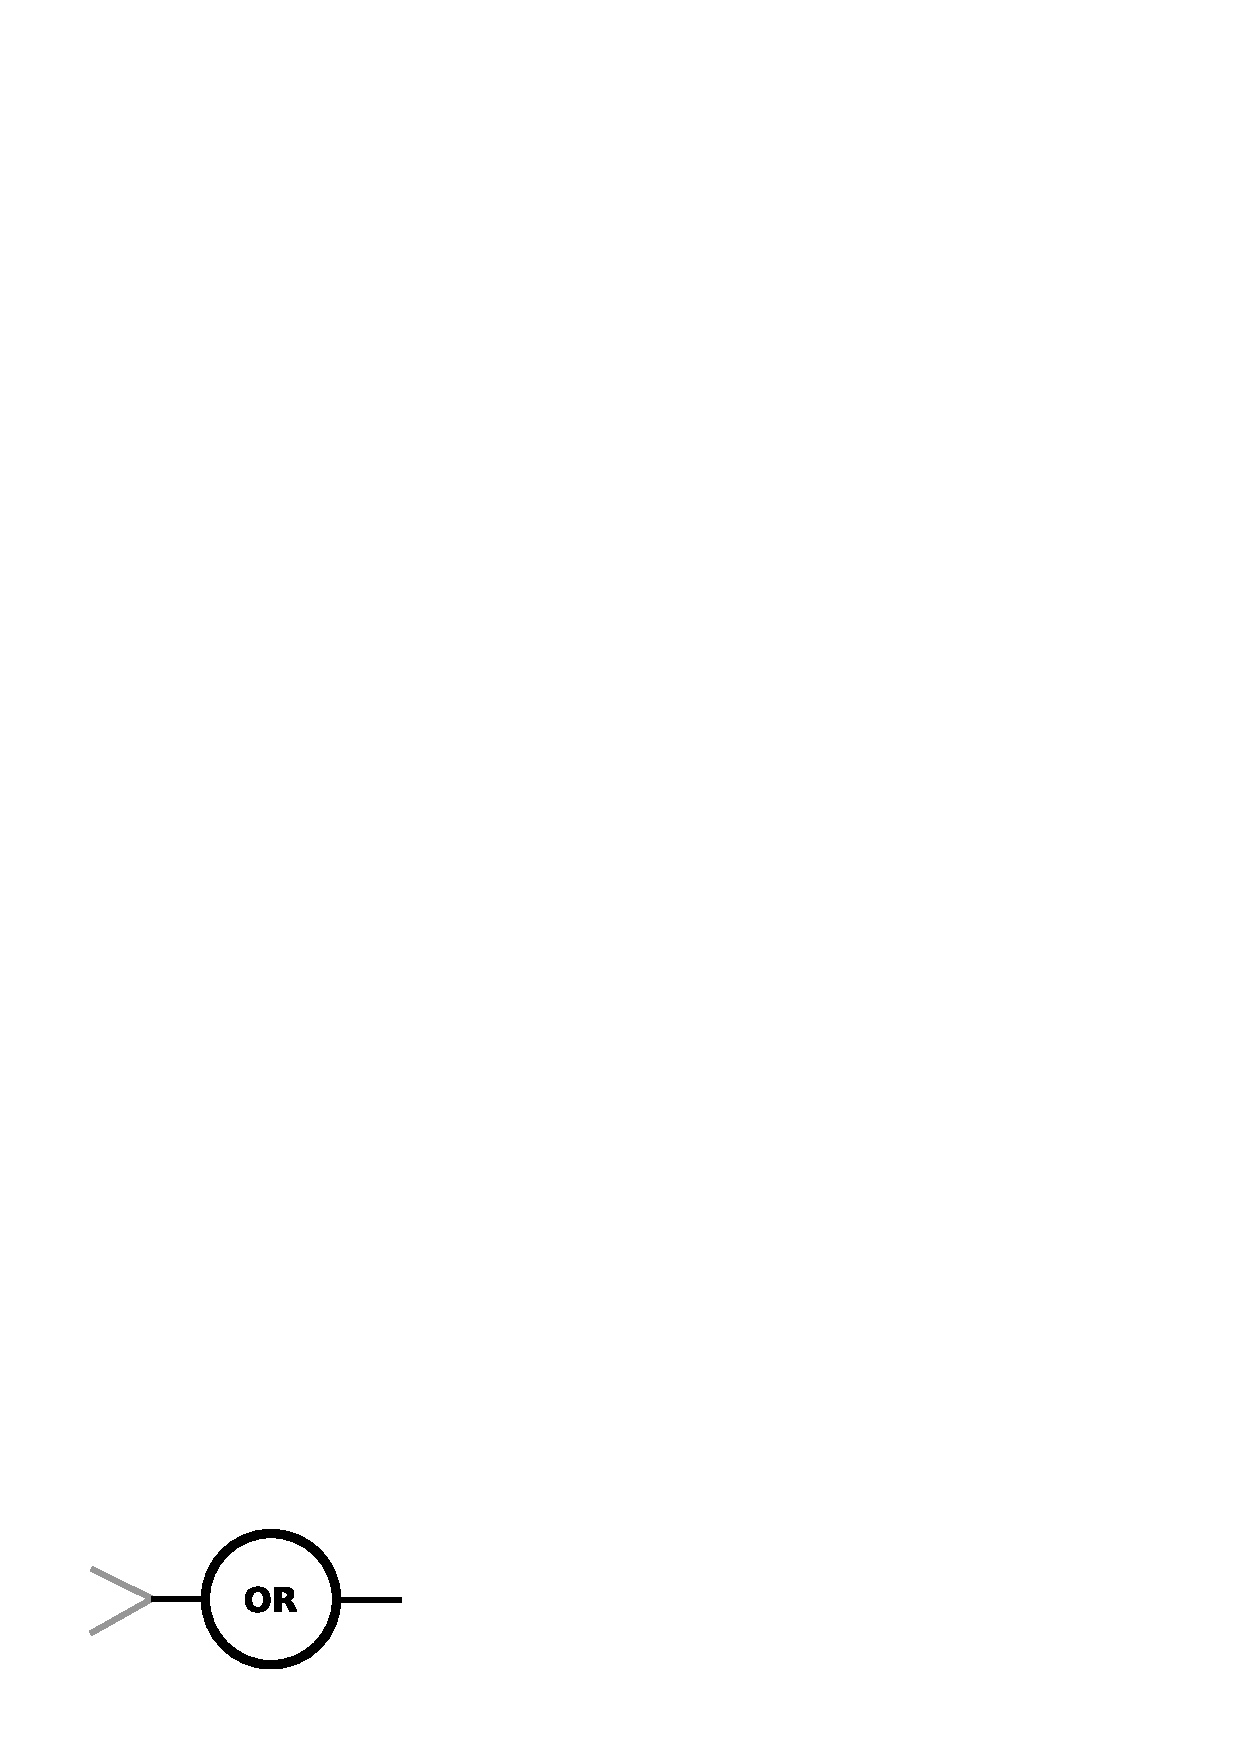
\includegraphics[scale = 1]{images/build/or.pdf}
  \caption{The \AF glyph for \glyph{or}. Only two inputs are represented, but more would be allowed.}
  \label{fig:af:or}
\end{figure}


\begin{figure}[H]
  \centering
  \includegraphics[scale = 0.8]{images/build/or_example.pdf}
  \caption{An example, taken from \fig{af:1}, of the \glyph{or} logical operator, where the activity from \glyph{"Genes for brown fat energy dissipation"} is positively influenced by either the \glyph{PPAR delta} activity or an \glyph{unspecified transcription factor} activity.}
  \label{fig:af:ex-or}
\end{figure}

\subsection{Glyph: \glyph{Not}}
\label{sec:af:not}

The output of a \glyph{not} glyph is True if its input is False, and False otherwise.

\begin{glyphDescription}
 \glyphSboTerm SBO:0000238 ! not.
 \glyphIncoming One \glyph{logic arc} (\sect{af:logicArc}).
 \glyphOutgoing  One \glyph{logic arc} (\sect{af:logicArc}) or one of the influence arcs (\sect{af:arcs}).
 \glyphContainer A \glyph{not} operator is represented by a circular shape containing the word ``NOT''.
The shape is linked to two ports, that are small arcs attached to the centres of opposite sides of the shape, as shown in \fig{af:not}.
 \glyphLabel None.
 \glyphAux None.
 \end{glyphDescription}

\begin{figure}[H]
  \centering
  \includegraphics[scale = 1]{images/build/not.pdf}
  \caption{The \AF glyph for \glyph{not}.}
  \label{fig:af:not}
\end{figure}

\begin{figure}[H]
  \centering
  \includegraphics[scale = 0.8]{images/build/not_example.pdf}
  \caption{An example of the \glyph{not} logical operator, where the activity of \glyph{NR1D1} has a negative influence on the activity of \glyph{Cdkn1a} taking place in the regulation of the circadian clock.}
  \label{fig:af:ex-not}
\end{figure}

%%%%%%%%%%%%%%%%%%%%%%%%%%%%%%%%%%%%%%%%%%%%%%%%%%%%%%%%%%%%%%%%%%%%%%
%%                     delay
%%%%%%%%%%%%%%%%%%%%%%%%%%%%%%%%%%%%%%%%%%%%%%%%%%%%%%%%%%%%%%%%%%%%%%

\subsection{Glyph: \glyph{Delay}}\label{sec:delay}

The \glyph{delay} glyph represents that the input, connected via a logic arc from a \glyph{BA} or the output of another logical operator, does not produce its influence immediately on the target activity.


\begin{glyphDescription}
 \glyphSboTerm SBO:0000225 ! delay.
 \glyphIncoming One \glyph{logic arc} (\sect{af:logicArc}).
 \glyphOutgoing  One \glyph{logic arc} (\sect{af:logicArc}) or one of the influence arcs (\sect{af:arcs}).
 \glyphContainer A \glyph{delay} operator is represented by a circular shape containing the symbol ``$\uptau$`` (letter ``tau'' of the Greek alphabet).
The shape is linked to two ports, that are small arcs attached to the centres of opposite sides of the shape, as shown in \fig{af:delay}.
 \glyphLabel None.
 \glyphAux None.
\end{glyphDescription}

\begin{figure}[H]
  \centering
  \includegraphics[scale = 0.6]{images/build/delay.pdf}
  \caption{The \AF glyph for \glyph{delay}.}
  \label{fig:af:delay}
\end{figure}

\begin{figure}[H]
  \centering
  \includegraphics[scale = 0.8]{images/build/delay_example.pdf}
  \caption{An example of the \glyph{delay} logical operator, where the activity of \glyph{p21} is positively influenced after a delay by the activity of \glyph{p53}, modelling the time-dependent transcriptional activation of p21 by p53.}
  \label{fig:af:ex-or}
\end{figure}
 

\section{Logic arc}
\label{sec:logic_arc}
%%%%%%%%%%%%%%%%%%%%%%%%%%%%%%%%%%%%%%%%%%%%%%%%%%%%%%%%%%%%%%%%%%%%%%
%%                     Logic arc
%%%%%%%%%%%%%%%%%%%%%%%%%%%%%%%%%%%%%%%%%%%%%%%%%%%%%%%%%%%%%%%%%%%%%%

\subsection{Glyph: \glyph{Logic arc} }\label{sec:af:logicArc}

\glyph{Logic arc} is used to represent the fact that an activity influences the outcome of a logic operator.

\begin{glyphDescription}
 \glyphSboTerm SBO:0000398 ! logical relationship.
 \glyphOrigin Any \glyph{biological activity} (\sect{af:biologicalActivity}) or any \glyph{logical operator} (\sect{af:logic}).
 \glyphTarget Any \glyph{logical operator} (\sect{af:logic}).
 \glyphEndPoint No symbol is used to represent the end of a logic arc.
 \end{glyphDescription}

\begin{figure}[H]
  \centering
  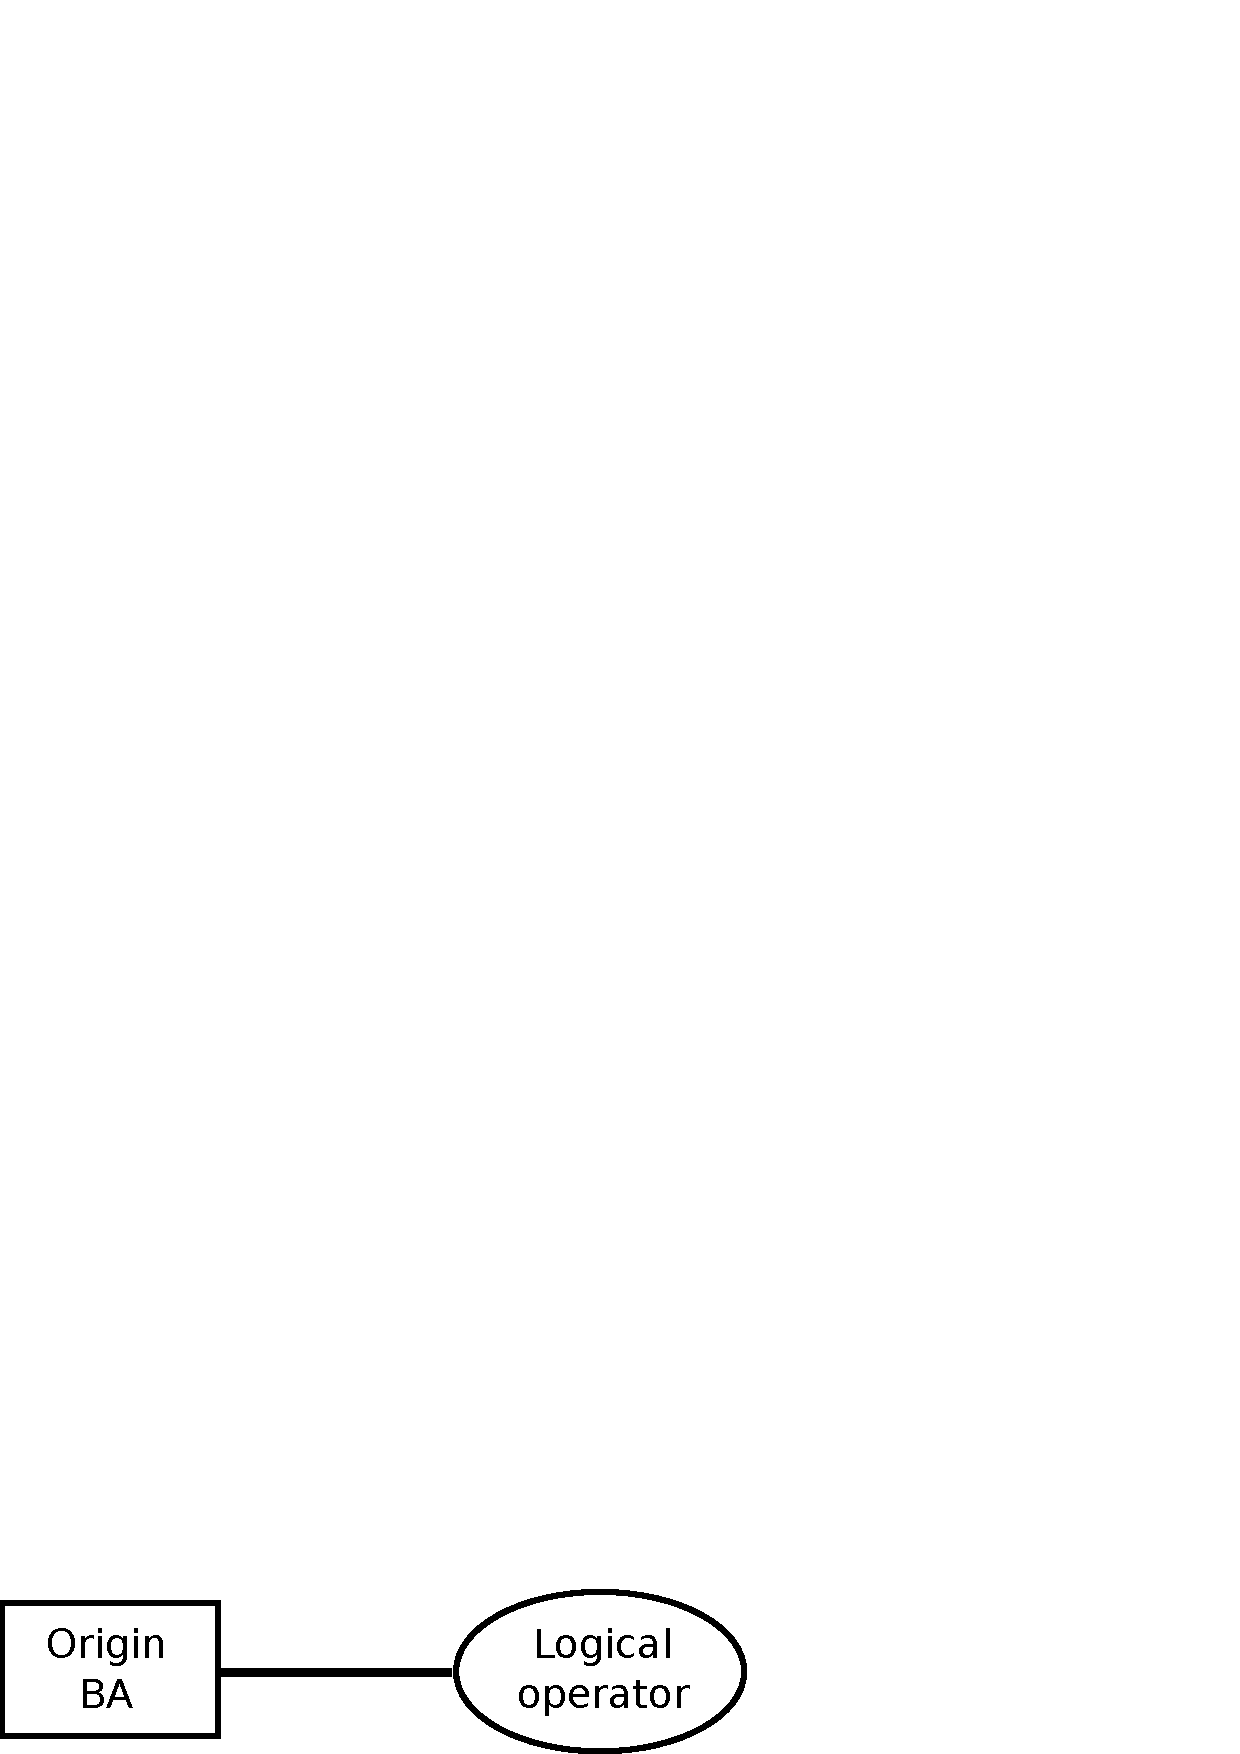
\includegraphics[scale = 0.4]{images/build/logicArc.pdf}
  \caption{The \AF glyph for \glyph{logic arc}. BA = biological activity}
  \label{fig:logicArc}
\end{figure}


\section{Annotating nodes and arcs}
%%%%%%%%%%%%%%%%%%%%%%%%%%%%%%%%%%%%%%%%%%%%%%%%%%%%%%%%%%%%%%%%%%%%%%
%%                     Annotation
%%%%%%%%%%%%%%%%%%%%%%%%%%%%%%%%%%%%%%%%%%%%%%%%%%%%%%%%%%%%%%%%%%%%%%

\subsection{Glyph: \glyph{Annotation}}
\label{sec:annotation}

\SBGNAFLone defines a glyph to add additional information to a map, that does not modify the semantics of the graph. This glyph can be used to add free text, or links to external information.

\begin{glyphDescription}

\glyphSboTerm SBO:0000550 ! annotation

\glyphIncoming None.

\glyphOutgoing None.

\glyphContainer An \glyph{annotation} is represented by a rectangular container with a folded corner, as illustrated in \fig{annotation}. This container is linked to the annotated element with a callout. The link ends up on the border of the annotated element.

\glyphLabel An \glyph{annotation} contains information placed in an unbordered box containing a string of characters.  The characters can be distributed on several lines to improve readability, although this is not mandatory.  The label box must be attached to the centre of the container. The label may spill outside of the container. 

\glyphAux None.
\end{glyphDescription}

\begin{figure}[H]
  \centering
  \includegraphics[scale = 1]{images/build/annotation.pdf}
  \caption{The \AF glyph for \glyph{annotation}.}
  \label{fig:annotation}
\end{figure}


\section{Referring to other nodes}
\label{sec:ref_nodes}



\input{src/tag.tex}
%%%%%%%%%%%%%%%%%%%%%%%%%%%%%%%%%%%%%%%%%%%%%%%%%%%%%%%%%%%%%%%%%%%%%%
%%                     Equivalence Arc
%%%%%%%%%%%%%%%%%%%%%%%%%%%%%%%%%%%%%%%%%%%%%%%%%%%%%%%%%%%%%%%%%%%%%%

\subsection{Glyph: \glyph{Equivalence arc} }\label{sec:equivalenceArc}

\glyph{Equivalence Arc} is used to represent the fact that all activities or compartments marked by a \glyph{tag} are equivalent. In an \AFm, it is used to show that an AN in a submap and another AN in the main map are equivalent.

\begin{glyphDescription}
 \glyphSboTerm Not applicable.
 \glyphOrigin Any \glyph{Activity node} (\sect{af:ANs}) or any \glyph{compartment}.
 \glyphTarget \glyph{Tag} or \glyph{Submap terminal}.
 \glyphEndPoint No symbol is used to represent the end of an \glyph{equivalence arc}.
 \end{glyphDescription}

\begin{figure}[H]
  \centering
  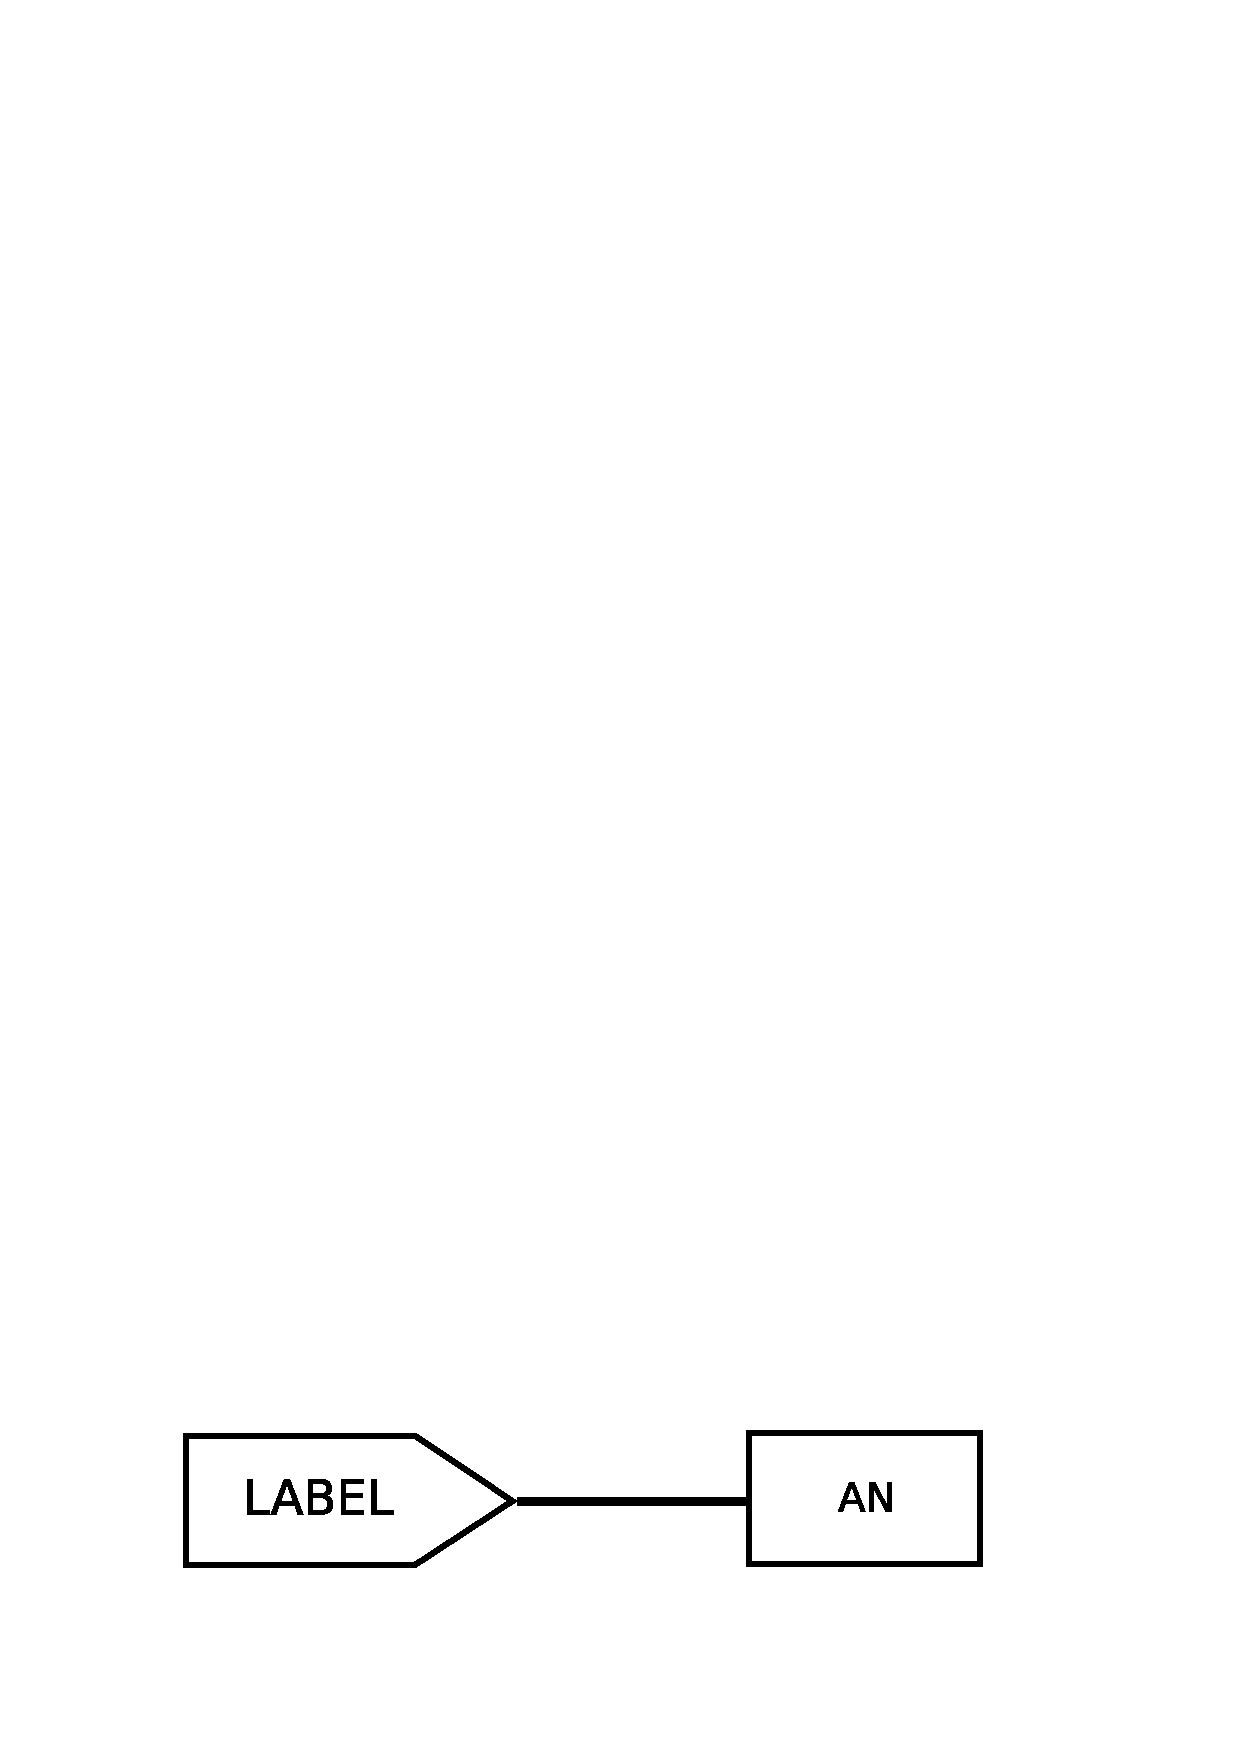
\includegraphics[scale = 0.4]{images/build/equivalence.pdf}
  \caption{The \AF glyph for \glyph{Equivalence arc}.}
  \label{fig:equivalence}
\end{figure}


\section{Encapsulation nodes}
\subsection{Glyph: \glyph{Submap}}
\label{sec:submap}

\begin{glyphDescription}

\glyphSboTerm To be determined.

\glyphContainer The \glyph{submap} is represented as a square box to remind the viewer that it is fundamentally a process.

\glyphLabel The identification of the \glyph{submap} is carried by an unbordered box containing a string of characters.  The characters may be distributed on several lines to improve readability, although this is not mandatory.  The label box has to be attached to the center of the container box.

\end{glyphDescription}



